\documentclass[a4paper,10pt]{amsart}
\usepackage[utf8]{inputenc}
\usepackage{amsmath}
\usepackage{amssymb}{}
\usepackage{amsthm}
\usepackage{enumerate}
\usepackage{hyperref}
\usepackage{listings}
\usepackage{booktabs}
\usepackage{siunitx}
\usepackage{graphicx}
\usepackage[numbers, comma, sort&compress]{natbib}
\usepackage{cleveref}
\begin{document}
    \author{SDIV, FPA, DGS, GASV}
    \title{Some fucking title}
    \maketitle

    \begin{abstract}
    	BACKGROUND.
    	CONTRIBUTION.
    	IMPLICATIONS-
    \end{abstract}

    \section{Introduction}
    \section{Model Formulation}
        \paragraph{Uncontrolled dynamics}
        We split the the constant population $N$ in a base SEIR 
        structure
        with segregation infected classes according with 
        manifestation  of symptoms.
        We also postulate the extra state $Y_{I_S}$ to fit commulative 
        symptomatic cases reported in the databases from Mexico city
       	during the exponential grow phase. Our dynamics reads
        \begin{equation}
        	\label{eqn:base_dynamics}
            \begin{aligned}
            	L' & = \theta \mu N^{\star}
                	-\epsilon \lambda L - \delta_L L - \mu L,
            	\\
            	S' & =
                	(1 - \theta)\mu N^\star + \delta_L   
                	- (\lambda + \mu) S,
            	\\
            	E' & =
                	\lambda (\epsilon L + S) - (\kappa + \mu) E,
            	\\
            	I_S' & =
                	p \kappa E - (\gamma_S + \delta_H + \mu_{I_S} + \mu) I_S,    
            	\\
            	I_A' &=
                	(1 - p) \kappa E - \gamma_A I_A - \mu I_A,
            	\\
            	H' &=
                	\delta_H I_S - (\gamma_H + \mu_H) H - \delta_H H - \mu H,
            	\\
            	R' & =
                	\gamma_S I_S + \gamma_A I_A + \gamma_H H - \mu R,
            	\\
            	D' &=
                	\mu_{I_S} I_S + \mu_H H,
            	\\
            	\frac{dY_{I_S}}{dt} &  = p \kappa E, 
            	\\
            	\lambda &:=
                	\frac{\beta_A I_A + \beta_S I_S}{N^{\star}},
            	\\
            	N^{\star}(t) &=
                	L + S + E + 
               	 	I_S + I_A +
                	H + R .
            \end{aligned}
        \end{equation}
         See table[*] for notation and values.
         \begin{table}[h!]
    \begin{tabular}{>{\centering}p{0.2\textwidth}p{0.6\textwidth}}
			\toprule
			Parameter & Description
      \\
      \midrule
			$\mu$ &  
				Death rate
			\\
            $\beta_S$ & 
            	Infection rate between susceptible and symptomatic infected
			\\
            $\beta_A$ & 
            	Infection rate between susceptible and asymptomatic infected
			\\
            $\lambda_V$ & 
            	Vaccination rate
			\\
            $\delta_{V}^{-1}$ & 
            	Immunity average time by vaccination
			\\
            $\varepsilon$ &  
            	Vaccine efficiency
			\\
            $\kappa^{-1}$ & 
            	Average incubation time   
            \\
			$p$ & 
				New asymptomatic generation proportion  
			\\			
		    $\theta$ & 
            	Proportion of individuals under lockdown 
            \\ 
            $\gamma_{S}^{-1}$ &  
            	Average output time of symptomatic individuals due to recovery
            \\
			$\gamma_{A}^{-1}$ & 
				Recovery average time of asymptomatic individuals  
			\\
			$\gamma_{M}^{-1}$ & 
				Recovery average time by medication
			\\
			$\gamma_{H}^{-1}$ & 
				Recovery average time by hospitalization
			\\ 					 
            
            $\delta_{R}^{-1}$ &  
            	Immunity average time by disease 
            \\
      	\bottomrule
		\end{tabular}
  		\caption{
  			Parameters definition of model in 
  			\cref{eqn:base_dynamics}.}\label{table1}
	\end{table}

        \begin{figure}[htb]
        	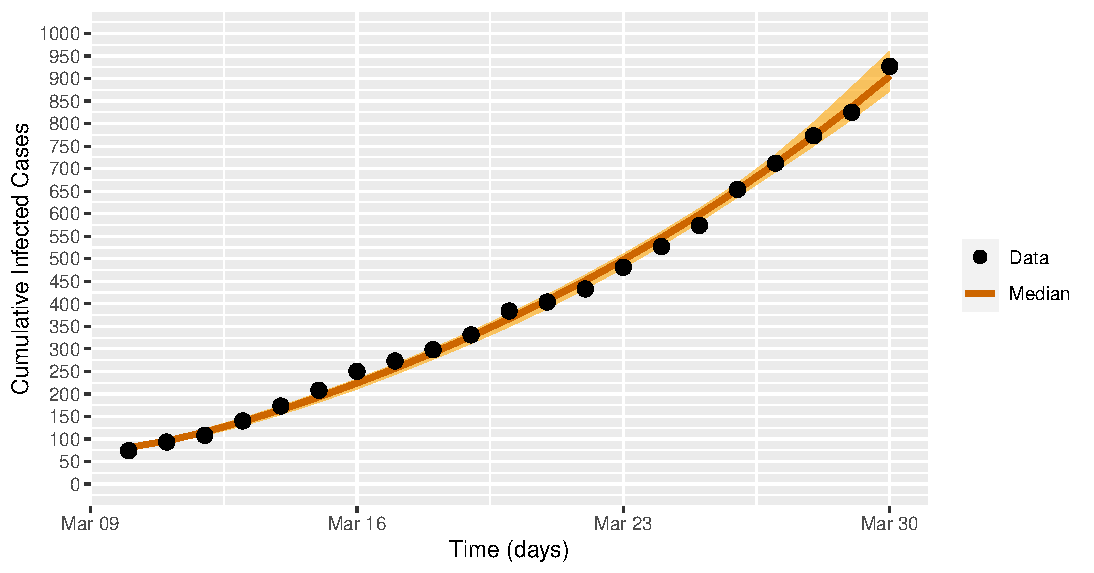
\includegraphics[width=\textwidth]{./cdmx_CIs_data_begining_fit}
        	\caption{%
        		Fit of diary new cases of Mexico city
        		during exponential growth.
        	}
        \end{figure}



        \paragraph{Hypothesis} We consider that susceptible individuals become
        infected when they are in contact with asymptomatic individuals and
        individuals with symptoms, we will propose that a proportion of
        asymptomatic individuals have a way to get relief and not die. A
        proportion of individuals infected with symptoms may die from the
        disease or may be relieved.

        	We callibrate parameters of our base dynamics in \eqref{eqn:base_dynamics}
        via Multichain Montecarlo (MCMC). To this end, we assume that the comulative 
        incidence of new infected symptomatic cases $CI_S$ 
        follows a Poisson distribution with mean $\lambda_t = IC_s(t)$. Further,
        following [] we postulate priors for $p$ and $\kappa$
        \begin{equation}
        	\label{eqn:boservation_model}
        	\begin{aligned}
        		Y_t & \sim Poisson(\lambda_t),
        		\\
        		\lambda_t 
        			&=
        			\int_{0}^t p \delta_e E ,
        		\\
        			& p \sim \text{Uniform} (0.3, 0.8),
        		\\
        			& \kappa \sim \text{Gamma}(10, 50).
        	\end{aligned}
        \end{equation}

    Ussing the reproductive number definition of VanDenDrishe, we obtain
	\begin{equation*}
		\label{eqn:reproductive_number}
		R_0 := 
			\frac{
				N^{*}(
					\beta_S p 
					\kappa + 
					\beta_A 
					\kappa(1-p) )
			}{
				(\mu - \kappa)( \gamma_S + \mu_{I_s} + S_A + \mu) 
				N^* \mu
			}
	\end{equation*}


        Figure [...] displays data of coumulative confirmed cases of COVID-19 of
    Mexico city, and the fitt of our model in 
    \cref{eqn:base_dynamics,eqn:boservation_model}.
    
    \paragraph{Controlled Model}
    We model vaccination, treatment and lockdown as a optimal control problem.
     According to dynamics in equation \eqref{model1}, we modulate the vaccination rate by 
a time-dependent control signal  $u_V(t)$. We add  compartment $X$ to count all the vaccine
applications of susceptible, exposed, asymptomatic and
recovered individuals. This process is modeled by
\begin{equation}
    \label{eqn:counter}
      X'(t) =
        (\lambda_V + u_V(t))(S + E + I_A + R)
\end{equation}
and describes the number of applied vaccines at time $t$.
 
Consider
  {$${x(t):= (S,E,I_S,I_A,R,D,V,X)^{\top}(t)}$$} and control signal
  $u_v(\cdot)$. We quantify the cost and reward of a vaccine strategy 
  policy via the penalization functional
  \begin{equation}
    \label{eqn:cost_functional}
    J(u_V):=
      \int _0 ^ T
      a_S I_S + a_d D +
      \frac{1}{2}
      %\left(
        c_V u_v^2
        % + c_T u_T^2
      %\right)
      ds.
  \end{equation}
  In other words, we assume in functional $J$ that pandemic cost is proportional to the
  symptomatic and death reported cases and that a vaccination policy
  implies quadratic consumption of resources.

  Further, since we aim to simulate vaccination policies at different coverage
  scenarios, we impose the vaccination counter state's final
  time condition $X(T)$
  \begin{equation}
    \begin{aligned}
      x(T) &= (\cdot, \cdot, \cdot, \cdot, \cdot, X(T))^{\top},
      \in \Omega
      \\
      X(T)
        &= x_{cover age},
      \\
      x_{coverage}
        & \in
        \left \{
          \text{Low(0.2)},\text{Mid(0.5)}, \text{High(0.8)}
        \right \} .
    \end{aligned}
  \end{equation}
  Thus, given the time horizon $T$, we impose that the last fraction of
  vaccinated populations corresponds to 20\%, 50\% or 80\%, and
  the rest of final states as free. We also impose the path constraint
  \begin{equation}
    \label{eqn:path_constrain}
    \Phi(x,t):= \kappa I_S(t) \leq B,
    \qquad \forall t \in [0, T],
  \end{equation}
  to ensure that healthcare services will not be overloaded. Here $\kappa$
  denotes hospitalization rate, and $B$ is the load capacity of a
  health system.

Given a fixed time horizon and vaccine efficiency, 
we estimate the constant vaccination rate as the solution of
\begin{equation}
    x_{coverage} = 1 - \exp(-\lambda_v T).
\end{equation}
 That is, $\lambda_v$ denotes the constant rate
to cover  a fraction $x_{coverage}$ in time horizon $T$. 
Thus, according to this vaccination rate, we postulate a policy $u_v$ that 
modulates vaccination rate according to $\lambda_V$ as a baseline. That is,
optimal vaccination amplifies or attenuates the estimated baseline 
$\lambda_V$ in a interval $[\lambda_v^{\min}, \lambda_v^{\max}]$ 
to optimize functional $J(\cdot)$\textemdash minimizing 
symptomatic, death reported cases and optimizing resources.

    Our objective is minimize the cost functional
  \eqref{eqn:cost_functional}\textemdash over an appropriated functional
  space\textemdash subject to the dynamics in equations \eqref{model1} and \eqref{eqn:counter},
  boundary conditions, and the path constrain in \eqref{eqn:path_constrain}.
  That is, we search for vaccination policies $u_V(\cdot)$, which
  solve the following optimal control problem (OCP)

    \section{SEIR version}
       Here we propose a SEIR structure which considers hospitalized
    compartment $ H $. To overcome stability issues we also consider
    vital dynamics.
    \begin{equation}
        \label{eqn:vital_dynamics}
        \begin{aligned}
            \min_{u \in \mathcal{U}} J(u) & :=
            \int_{0}^T
                % \left(
                    a_{I_S} I_S
                    + a_{H} H
                    + a_{D} D
                  %  +
                  %  \frac{a_{L}}{2}  u_L ^ 2
                  %  +
                  % \frac{a_{V}}{2} u_V ^ 2
                  %  +
                  %  \frac{a_{H}}{2} u_H ^ 2
                  %  +
                  %  \frac{a_{M}}{2} u_M ^ 2
                %\right)
                dt
            \\
            \text{s. t.} &
            \\
            L' & =  \theta \mu N^{\star}
                -\epsilon \lambda L - u_L(t) L - \mu L
            \\
            S' & = 
                (1 - \theta) \mu N^\star 
                + u_L(t) L 
                + (1 - \widehat{q}) \gamma_V V 
                + \delta_v V 
                + \delta_R R
            \\
                & \qquad - 
                \left[
                	\lambda + (\lambda_V + u_V(t)) + \mu
                \right] S 
            \\
            E' &= 
                \lambda (\epsilon L + (1-\varepsilon) V + S) 
                - (\kappa + \mu) E
            \\
            I_S' &= 
                p \kappa E 
                + (1 - q) \gamma_M M(t)
                - (\gamma_S + \mu_{I_S} + \delta_H + u_M(t) + \mu) I_S
            \\
            I_A' &= 
                (1 - p) \kappa E - (\gamma_A + \mu) I_A
            \\
            M' &= 
                u_M(t) I_S - (\gamma_M + \mu ) M
            \\
            H' &= 
                \delta_H I_S - (\gamma_H + \mu_H + \mu) H 
            \\
            R'  &= 
                \gamma_S I_S + \gamma_A I_A + \gamma_H H + q \gamma_M M
                - (\delta_R + \mu) R
            \\
            D' &= 
                \mu_{I_S} I_S + \mu_H H
            \\
            V' &= 
                (\lambda_V + u_V(t)) S  
                - \left[
                	(1 - \varepsilon) \lambda
                	+ \delta_V
                	+ \mu
                \right ] V
            \\
            \\
            \frac{dX_{vac}}{dt}
            	&=
            	(u_V(t) + \lambda_V)
            	\left[
            		S + E + I_A + R - (\gamma_S I_S + \gamma_H H)  
            	\right]
            \\
            \frac{d Y_{I_S}}{dt}
            	& = p \kappa E
            \\
            \lambda &:=
                \frac{\beta_A I_A + \beta_S I_S}{N^{\star}}
            \\
            N^{\star}(t) &=
                L + S +E + I_S + I_A +
                M + H + R + V
        \end{aligned}
    \end{equation}
	
    \paragraph{Bayesian estimation}
    
    \section{Parameters}
        \begin{table}
        \begin{tabular}{@{}llc@{}} 
        \toprule
            Parameter
            &   \centering{Median}
            &   Reference
            \\
            \midrule
                $\beta_S$
                & \num{8.690483e-01}
                & $*$
            \\
                $\beta_A$
                & \num{7.738431e-01}
                & $*$
            \\
                $\kappa$
                & \num{2.143749e-01}
                & $*$
            \\
                $p$
                & \num{4.387130e-01	}
                & $*$
            \\
                $\delta_H$
                &\num{4.603172e-01}
                & $*$
            \\
                $\mu$
                &
                $
                    0.000039139
                $
                & $**$
            \\
                $\mu_{I_S}$
                & $\num{5.691990e-02}$
                & $*$
            \\
                $\mu_{H}$
                & $\num{3.280390e-02}$
                & $*$
            \\
                $\gamma_S$
                & \num{1.197828e-01}
                & $*$
            \\
                 $\gamma_A$
                 & \num{5.113880e-01}
                 & $*$
            \\
               $\gamma_H$
                & \num{4.880279e-01}
                & $*$
            \\
                $N$
                 & \num{8918653}
                 & $**$
            \\
                $S_0$
                 & $N - (E_0 + I_{S_0} + I_{A_0})$
                 &
            \\
                $E_0$
                 & \num{1388}
                 & $*$
            \\
                $I_{S_0}$
                & $\num{22}$
                & $***$
            \\
                $I_{A_0}$
                & $\num{1595}$
                & $*$
            \\
                $H_0$
                & \num{0}
                & $**$
            \\
                $R_0$
                & \num{0}
                & $**$
            \\
                $D_0$
                & \num{0}
                & $**$
            \\
            \bottomrule
        \end{tabular}
    \end{table}
    %
    \section{Optimal control problem}
    
    \section{Numerical Results}
    
    \paragraph{Bayesian}
        
    
    \section{Appendix}

Consider the following cost functional that we want to minimize
  \begin{equation}\label{costFunctional}
  \int_0^T C(t,X(t),u(t)) dt
  \end{equation}
subject to the dynamics
  \begin{equation}\label{dynamics}
  \dot{X}(t) = f(t,X(t),u(t)),  \qquad    0\leq t \leq T,
  \end{equation}
and the initial state $X(0)=x_0$. Let $t_0<t_1<\ldots <t_n$, with $t_0=0$ and $t_n=T$, be a partition of the interval $[0,T]$. We consider {\it piecewise constant controls} $\tilde{u}$ of the form 
         \begin{equation}\label{PieceConstCont}
  \tilde{u}(t) = a_j\qquad t_j\leq t < t_{j+1}  
         \end{equation}
 for $j=0,\ldots,n-1$.	

{\sc Assumption 1}. 


{\sc Assumption 2}. 

By Assumption 1, the system
    \[    \dot{X}(t) = f(t,X(t),a_0), \quad X(0)=x_0, \qquad    0\leq t \leq t_1,
  \]
has a unique solution $\tilde{X}_0(t;x_0,a_0)$ which is continuous in $(x_0,a_0)$.  Next, put $x_1:=\tilde{X}_0(t_1;x_0,a_0)$ and consider the system
    \[    \dot{X}(t) = f(t,X(t),a_1), \quad X(t_1)=x_1, \qquad    t_1\leq t \leq t_2,
  \]
which, again by Assumption 1, has a unique solution $\tilde{X}_1(t;x_1,a_1)$ continuous in $(x_1,a_1)$. By following this procedure, we end up having a recursive solution
	\[  \tilde{X}_{n-1}(t;x_{n-1},a_{n-1}),\quad   x_{n-1}:=\tilde{X}_{n-2}(t_{n-1};x_{n-2},a_{n-1}),     \qquad    t_{n-1}\leq t \leq T. \]

Thus, for a control $\tilde{u}$ of the form \eqref{PieceConstCont} and the corresponding solution path $\tilde{X}$, we have
	\[  
	\int_0^T C(t,\tilde{X}(t),\tilde{u}(t)) dt   =     \sum_{j=0}^{n-1}   \int_{t_j}^{t_{j+1}} C(t,\tilde{X}_j(t),a_j) dt.
	\] 
Notice that each $\tilde{X}_j$ is a continuous function of $(a_0,\ldots,a_j)$	 and $x_0$. Therefore, by Assumption 2, the mapping 
		\[  
		(a_0,\ldots,a_{n-1}) \mapsto  \sum_{j=0}^{n-1}   \int_{t_j}^{t_{j+1}} C(t,\tilde{X}_j(t),a_j) dt
		\]
is continuous.	

    
    
    
    
    
    \nocite{*}
    \bibliography{NovelCovid19.bib}
    \bibliographystyle{plain}
\end{document}
